\documentclass[a4paper]{article}


\usepackage[T2A]{fontenc}
\usepackage[utf8]{inputenc}
\usepackage[english,russian]{babel}
\usepackage{graphicx}
\graphicspath{{pictures/}}
\DeclareGraphicsExtensions{.pdf,.png,.jpg}
\usepackage{amsmath, amsfonts, amssymb, amsthm, mathtools}

\author{Sergey}
\title{Линейная алгебра}
\date{\today}

\begin{document}

\maketitle

\newpage

\section{Лекция 1 Метод Гаусса}

$x_1....x_n$ - переменные
Линейное ураванение: $a_1x_1 + a_2x_2 + ... + a_nx_n = b$, $a_i$, $b_i$ - известные числа


\begin{equation*}
 \begin{cases}
 a_{11}x_1 + a_{12}x_2 + ... + a_{1n}x_n = b_1 \\
 a_{21}x_1 + a_{22}x_2 + ... + a_{2n}x_n = b_2 \\
   ..\\
   a_{n1}x_1 + a_{n2}x_2 + ... + a_{nn}x_n = b_n \\
 \end{cases}
\end{equation*}
$a_{ij} $ - клэффициенты уравнений
$b_n$ - правые части



Определение:\\
Если решение есть - то система называется совместной\\
Если решений нет - называется не совместной\\
Если решение есть и единственное - система называется опрделеленной\\

Пример:

\begin{equation*}
 \begin{cases}
   2x + 3y = 4
 \end{cases}
\end{equation*}
В таком случае пытаемся выразить одну переменную через другую.\\
Ответ: y - любое, x = $\frac{4-3y}{2}$\\

Определение: Матрица - это прямоугольная таблица, заполненная числами

\begin{equation*}
A = 
\begin{pmatrix}
  a_{11} ... a_{1n}\\
  ... ... ...\\
    a_{m1} ... a_{mn}\\
\end{pmatrix}
\end{equation*}
- Матрица коэффициентов системы линейых уравнений(СЛУ)
\begin{equation*}
A_2 = 
\begin{pmatrix}
  a_{11} ... a_{1n}  b_1\\
  ... ... ...\\
    a_{m1} ... a_{mn} b_m\\
\end{pmatrix}
\end{equation*}
- Расширеная матрица коэффициентов СЛУ


План решения СЛУ:
1) Ввести элементарные преобразования СЛУ (матриты $A_2$), которые не меняют множества решений СЛУ
2) Привести этими элементарными пребразрованиями к некому "хорошему" виду
3) Решить конечную систему в этом "хорошем" виде


Определение:
Две СЛУ называются  эквивалентными, если множества решений совпадают.

I тип элементарного преобразования:
i-е уравнение, умноженное на число $\lambda$, прибавляем к j уравнению (прибавляем левую часть к левой, а правую часть к правой. (i-е уравнение не меняем)

Пример: умножим первую строчку на 2 и прибавим к 3 строчке


\begin{equation*}
\begin{pmatrix}
  1, 2, 3, 4, 5 \\
  6, 7, 8, 9, 10\\
  2, 1, 2, 1, 0
\end{pmatrix} = 
\begin{pmatrix}
  1, 2, 3, 4, 5\\
  6, 7, 8, 9, 10\\
  4, 5, 8, 9, 10
\end{pmatrix}
\end{equation*}

II тип элементарного преобразования:\\
Берем i и j строчки и меняем их местами


III тип элементарного преобразования:\\
i строчку умножаем на $\lambda, \lambda \neq 0$


Теорема: Элементарные преобразования преодят СЛУ в эквивалентную.

Доказательство:\\
 ( отложили на конец лекции, основная идея - есть обратные преобразования)


Что такое "хороший" вид:
Определение: "Лидер строки"(ведущий элемент) строки матрицы - самое левое не нулевое число

\begin{equation*}
\begin{pmatrix}
  3 , 0, 2, 4 \\
  0, 0, 1, 2\\
  0, 4, 3, 0
\end{pmatrix}
\end{equation*}



Определение: Матрица имеет ступенчатый вид, если:
- Все нулевые строчки находятся снизу
- Номера столбцов лидеров образуют возрастающую последовательность
если все нулевые строчки находятся снизу
\begin{equation*}
\begin{pmatrix}
  3 , 0, 2, 4 \\
  0, 0, 1, 2\\
  0, 0, 0, 1\\
    0, 0, 0, 0\\
\end{pmatrix}
\end{equation*}

Нужно привести матрицу $A_2$  к ступенчатуму виду.
1. Берем столбцы, пока не находим не нулевой столбец i
2. Ставим строчку с элементом первым не нулевым элементом ($a_{ij}$) в столбце i на верх через преобразование 2 типа
3. за счет элементарного преобразования 1 типа обнуляем все элементы кроме $a_{ij}$
4. Переходим к матрице ниже на одну строчку и правее на один столбец.

Определене: Улучшенный ступенчатый вид - это ступунчатый вид, все лидеры строк - единицы, над лидерами строк находятся нули

Алгоритм приведения к Уучшенному ступенчатому виду:
1. Умножим каждую строчку на $\frac{1}{a}$, где a - значение лидера строки
2. Идем по строкам снизу, обнуляем все элементы над лидерами строк

Определение: Прямой ход метода Гаууса (метод Гаусса)  - Приведение к (улучшенному) ступенчатому виду по алгоритму сверху.

Определение: Обратный ход метода Гаусса:
- Идем снизу верх
1. Смотрим на последнюю строку



Определение: экзотическое уравнение:

$0x +...+ 0x_{n}=  b, b \neq 0$



Теорема: для любого набора значений свободных переменных существует единственное значение главных переменных, дополняющих до решения




Преобразования I типа не меняют множество решений:\\
В результате сложения двух равенств получается верное равенство -> множество решений не уменьшилось.
\\При элементарном преобразовании 1 типа множество решений не меньше чем множество решений в исходной СЛУ.\\
Так как для любого преобразования 1 типа можно подобрать обратное преобразование 1 типа, Множество решений измененной системы не увеличивается
\\
\\

\section{Лекция 2 Действия с матрицами}


A - матрица m на n


\begin{equation*}
\lambda A =  
\begin{pmatrix}
  \lambda x_11 & .. & \lambda x_1n\\
    \lambda x_m1& ..& \lambda x_mn
\end{pmatrix}
\end{equation*}

\begin{equation*}
A =  
\begin{pmatrix}
   a_11 & .. & a_1n\\
     a_m1& ..&  a_mn
\end{pmatrix},
B =  
\begin{pmatrix}
   b_11 & .. & b_1n\\
     b_m1& ..&  b_mn
\end{pmatrix}
\end{equation*}

Сложение матриц: $A, B \in Mat_{nxm}$.\\
$A + B = C \in Mat_{nxm}$ \\
$c_{ij} = a_{ij} + b_{ij}$


Свойство введенных операций.\\
1) $(A + B) + C = A + (B + C)$ - Ассоциативность\\ ( $(a_{ij} + b_{ij}) + c_{ij} = (a_{ij} + (b_{ij} + c_{ij})$



1.1) Обобщенная ассоциативность:\\
$A_1 + A_2 + ... + A_k$ - результат одинаковый при любой расстановке скобок


2) $\alpha (\lambda A) =  \lambda (\alpha A)$


3) ($\alpha + \lambda) A =  \lambda A +  \alpha A$


4) $\lambda (A + B) =  \lambda A +  \lambda B$


5) $1 A  = A$


6) 

\begin{equation*}
0 =  
\begin{pmatrix}
   0 & .. & 0\\
     0& ..&  0
\end{pmatrix},
\end{equation*}


7) $A + B = B + A$


8) $-A: A + (-A) = 0$


Умножение матриц:

$$ A_{mxn} B_{nxk} = C _{mxk}$$

$ c_{ij} = \sum^n_{t=1}a_{it}b{tj}$



Свойства умножения матриц:

1) $(A * B) * C = A * (B * C)$

$$A B = J$$

$$d_{ij} = \sum^n_{t=1}a_{it}b{tj}$$

$$(A B) C = F$$

$$f_{pq} = \sum^k_{s=1}d_{ps}c_{sq} = \sum^k_{s=1}\sum^n_{t=1}a_{pt}b_{ts}c_{sq}$$


Для $A (B C) = L$ Сумма аналогична, поэтому $L = F$.

1.1) Общая ассоциативность: $A_1A_2..A_n$ - Не завистит от расстановки скобок.


2) A(B + C) = AB + AC Дистрибутивность.


3) $(A + B)C = AC + BC$


4) $(\lambda A)B = A(\lambda B) = \lambda (AB)$



5) Единичная матрица: $ 1A = A$.
\begin{equation*}
E =  
\begin{pmatrix}
   1 & .. & 0\\
     0& ..&  1
\end{pmatrix},
\end{equation*}



....\\
....\\
....\\


Тнаспонирование матриц:

$$A_{mn} -> B_{nm} = A^T$$
$$a_{ij} = b_{ji}$$

$$(PQ)^T = Q^TP^T$$

След матрицы - сумма ее диагональных элементов.

$$tr(A) = a{11} + a{22} + a{33} + ... + a{nn}$$

Теорема:
$$ tr(PQ) = tr(QP)$$





\section*{Лекция 6. Перестановки}


Опр. Перестановка длины n - переупорядоченный набор от 1 до n.

Например (2, 3, 7, 4, 6, 1, 7) - перестанока длинны 7.

Подстановка длинны n - это отображение  (биекция) $\sigma :{1,2,3,4,5,..n} /to {1,2,3,4,5,..n}$


Пример:

\begin{equation*}
\sigma = 
\begin{pmatrix}
	1 & 2 &3 & 4 & 5\\
	3 & 4 & 5 & 1 & 2\\	
\end{pmatrix}
=
\begin{pmatrix}
	2 & 3 &1 & 4 & 5\\
	4 & 5& 3 & 1 & 2\\	
\end{pmatrix}
\end{equation*}

Существует биекция между подстановками и перестановками.

Всего $n!$ престановок.


Произведение подстановок:

$$ \gamma = \delta \dot \sigma$$
$$ \gamma(i) = \delta \cdot \sigma(i) = \delta ( \sigma(i))$$
При перемножении начинаем с перестановки справа:

\begin{equation*}
\sigma \delta= 
\begin{pmatrix}
	1 & 2 &3 & 4 & 5\\
	3 & 4 & 5 & 1 & 2\\	
\end{pmatrix}
\cdot
\begin{pmatrix}
	1 & 2 &3 & 4 & 5\\
	2 & 1 &3 & 4 & 5\\
\end{pmatrix}
=
\begin{pmatrix}
	1 & 2 &3 & 4 & 5\\
	4 & 3 & 5 & 1 & 2\\	
\end{pmatrix}
\end{equation*}

$$ 1 \to 2 \to 4$$
$$ 2 \to 1 \to 3$$

Произведение перестановок не коммуникативно!
$$ \sigma \delta \neq \delta \sigma $$

Произведение перестановок ассоциативно.
$$ (\sigma \delta) \gamma = \sigma (\delta \gamma)$$
$$ (\sigma \delta) \gamma(x) = (\sigma \delta) (\gamma(x)) = \sigma (\delta (\gamma(x))))= $$
$$ =\sigma (\delta \gamma)(x) = \sigma (\delta\gamma(x)) = \sigma (\delta (\gamma(x))))$$


Тождественная перестановка id (единичная перестановка):

\begin{equation*}
id= 
\begin{pmatrix}
	1 & 2 &3 & 4 & 5\\
	1 & 2 &3 & 4 & 5\\
\end{pmatrix}
\end{equation*}

Обратная перстановка : $\sigma^{-1}$. Так как $\sigma$ - биекция, такая перестановка единственна.

(просто меняем местами верхний и нижний элемент)


\begin{equation*}
\sigma= 
\begin{pmatrix}
	1 & 2 &3 & 4 & 5\\
	4 & 3 & 5 & 1 & 2\\	
\end{pmatrix}
\end{equation*}
\begin{equation*}
\sigma ^{-1}= 
\begin{pmatrix}
	1 & 2 &3 & 4 & 5\\
	4 & 5 & 2 & 1 & 4\\	
\end{pmatrix}
\end{equation*}


$$\sigma \sigma^{-1} = id$$

\subsection*{Разложение в независимые циклы}

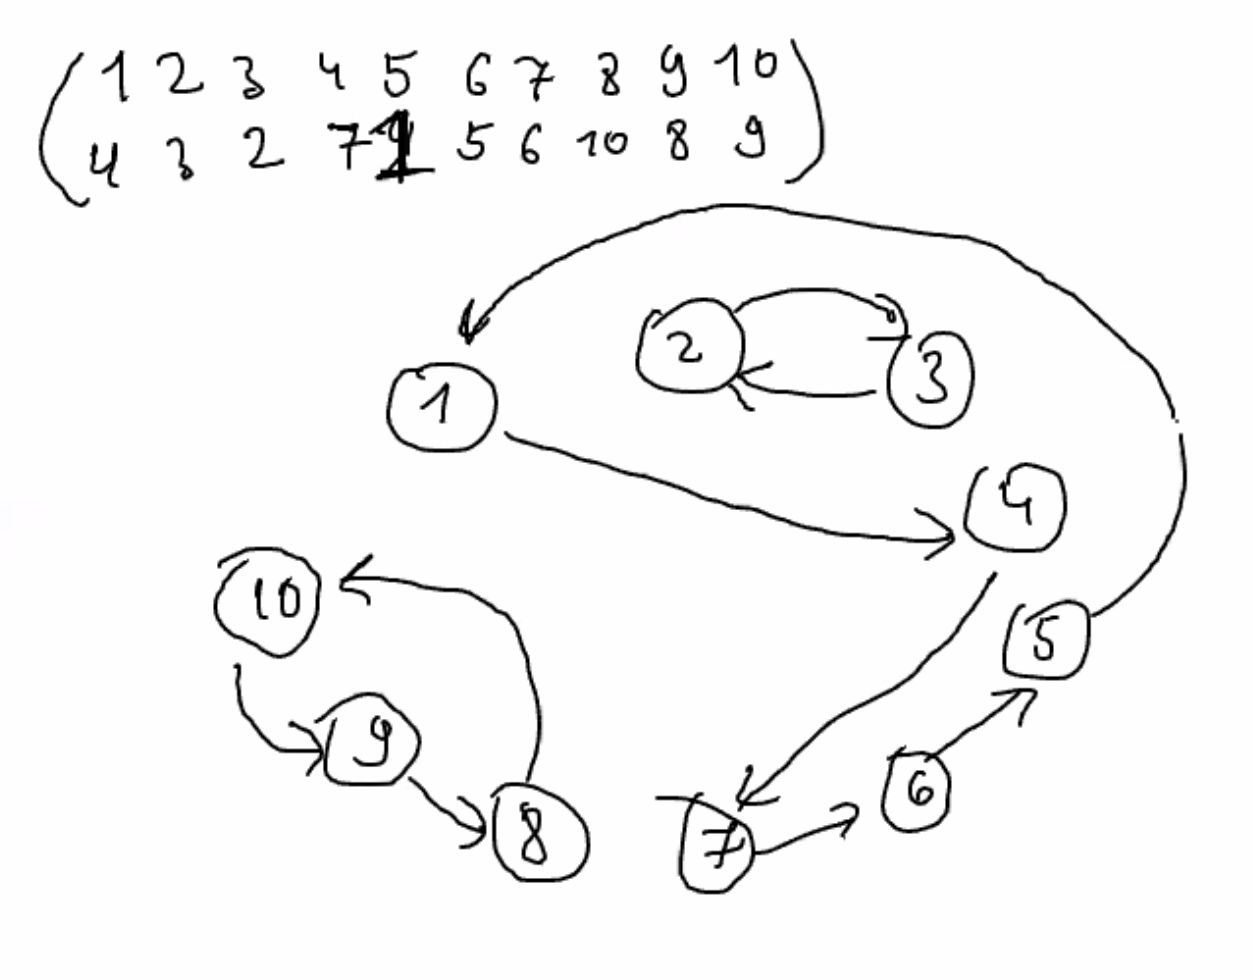
\includegraphics[width=12cm]{premutations_circle}


Лемма:ориентироанный граф, построенный по подстановке - это объединение нескольких не пересекающихся циклов.

Доказательство:из любой вершины выходит одна стрелка и входит одна стрелка.



\begin{equation*}
\begin{pmatrix}
	1 & 2 & 3 & 4 & 5 & 6 & 7 & 8 & 9 & 10\\
	4 & 3 & 2 & 7 & 1 & 5 & 6 & 10 & 8 & 9\\	
\end{pmatrix}
=
\begin{pmatrix}
	1 & 4 &7 & 6 & 5 
\end{pmatrix}
\begin{pmatrix}
	2 & 3
\end{pmatrix}
\begin{pmatrix}
	8 & 10 & 9
\end{pmatrix}
\end{equation*}


\begin{equation*}
\begin{pmatrix}
	2 & 3
\end{pmatrix}= 
\begin{pmatrix}
	1 & 2 &3 & 4 & 5\\
	1 & 3 &2 & 4 & 5\\
\end{pmatrix}
\end{equation*}


\subsection*{Возведение в степень}
\subsection*{Четность перестановок}








\begin{equation*}
 \begin{cases}
   
pass

 \end{cases}
\end{equation*}

\begin{equation*}
A = 
\begin{pmatrix}
  pass
\end{pmatrix}
\end{equation*}



\end{document}